\title{How to make a Linked List in C++}
\author{
        Jake Billings \\
        Department of Computer Science\\
        Rensselaer Polytechnic Institute\\
        Troy, NY
}
\date{October 1, 2018}

\documentclass[12pt]{article}

\usepackage{hyperref}
\usepackage{listings}
\usepackage{graphicx}
\graphicspath{ {./} }

\begin{document}
\maketitle

\begin{abstract}
	This article contains a brief description of and a tutorial for the creation of the linked list data structure. It is intended for fellow computer science students in a data structures course.
\end{abstract}

\newpage

\section{What is a Linked List?}
If you're reading this, there's a good chance that you're a computer science student just like me. In that case, you probably have a good idea of what a Linked List is, so I won't spend too much time explaining it. Here's a brief refresher:

According to \href{https://www.cs.cmu.edu/~adamchik/15-121/lectures/Linked Lists/linked lists.html}{this page from Carnegie Mellon Unversity} (CMU),

\begin{quote}
	A linked list is a linear data structure where each element is a separate object. Each element (we will call it a node) of a list is comprising of two items - the data and a reference to the next node. The last node has a reference to null. The entry point into a linked list is called the head of the list. It should be noted that head is not a separate node, but the reference to the first node. If the list is empty then the head is a null reference.
\end{quote}

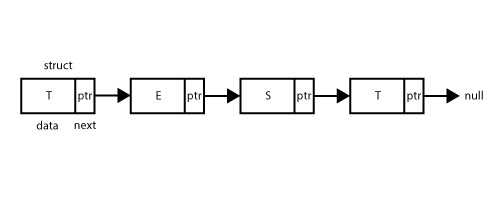
\includegraphics[width=\textwidth]{linked_list_diagram}

\paragraph{Why?}
	We use linked lists for their relatively quick insertion times. You'll see later. Inserting into a Linked List requires only a single O(1) operation. Linked Lists are not well-suited to applications where the end of the list is read frequently. Since lookup times near the end of the list are O(n) where n is the number of elements in the list, these lookups are inefficient compared to other data structures.

\newpage

\section{Implementation}

The following code listing will highlight the important pieces of a C++ linked list implementation:

\subsection{Node}

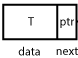
\includegraphics{node_diagram}

\begin{lstlisting}[language = C++]
template<typename T>

class Node {
private:
/**
* the actual data that this node holds
*/
T data;

/**
* a pointer to the next node in the linked list
*  this will be nullptr if this is the last node in the list
*/
Node *next;
public:
//getters, setters, and stream operators omitted for brevity
};
\end{lstlisting}

\newpage

\subsection{LinkedList Fields}

\begin{lstlisting}[language = C++]
template<typename T>
class LinkedList {
private:
/**
* head
*
* Node<T> pointer
*
* this is a pointer to the first node of the linked list
*/
Node<T> *head;
\end{lstlisting}

\paragraph{LinkedList}
In this example, the LinkedList class has one private field, which is the head pointer. The list manipulation functions in the LinkedList class all use this pointer to begin data access. No other references to elements of the list are stored.
\newpage

\subsection{Insert at Front}


\begin{lstlisting}[language = C++]
/**
* push_front()
*
* adds an element to the front of this linked list by wrapping it
* in a new node object, placing it on the heap,
*  and updating the head pointer
*
* @param  value the value to place into the LinkedList
* (type T from template)
*/
void push_front(T value) {
	//Allocate a new node on the heap that points
	//to the old head node
	Node<T> *n = new Node<T>(value, this->head);
	
	//Set head to point at the new node on the heap
	this->head = n;
}
\end{lstlisting}

\paragraph{push\_front()}
Inserting at the front of a LinkedList is easy. Just create a new node that points to the head pointer. Then, point the head pointer at the new node. This operation has complexity \textbf{O(1)}.

\newpage

\subsection{Insert at Back}


\begin{lstlisting}[language = C++]
/**
* push_back()
*
* adds an element to the back of this LinkedList by iterating
* through all the elements, then creating a new node,
*  placing it on the heap, then setting the next pointer of
* the last node
*/
void push_back(T value) {
//If the list is already empty, use the simpler algorithm
//from push_front to insert the
// value then return
if (this->head == nullptr) {
return this->push_front(value);
}

//Now, we can assume the head pointer is a node (not nullptr).
// We iterate until we find the last node
Node<T> *cur = this->head;
while (cur->getNext() != nullptr) {
cur = cur->getNext();
}

//Allocate a new node on the heap that points to nullptr
//(since it's the last element of the list)
Node<T> *n = new Node<T>(value, nullptr);

//Update the ptr of the node that used to be the last
//node to point at the new node
cur->setNext(n);
}

\end{lstlisting}

\paragraph{push\_back()}
Inserting at the back of a LinkedList is hard. You must follow every single pointer until you reach the end of the list. Then, you can point the final pointer at your new node. This operation has complexity \textbf{O(n)}.

\newpage

\subsection{Full Implementation}
Only a few functions are documented in this tutorial. I have a complete implementation available on GitHub. It contains operations for adding and removing elements at any position in the list. It also manages the allocation and freeing of memory in constructors and destructors. This implementation has been verified using automated testing.\\

\href{https://github.com/jake-billings/edu-csci2312/tree/master/hw06}{https://github.com/jake-billings/edu-csci2312/tree/master/hw06}

\newpage

\section{Additional Links}

\noindent
Other Projects: 
\href{https://github.com/jake-billings/}{https://github.com/jake-billings/}\\

\noindent
Data Structures: \href{https://github.com/jake-billings/edu-csci2421}{https://github.com/jake-billings/edu-csci2421}\\

\noindent
Medium: \href{https://github.com/jake-billings/edu-csci2421}{https://github.com/jake-billings/edu-csci2421}


\end{document}